
%(BEGIN_QUESTION)
% Copyright 2006, Tony R. Kuphaldt, released under the Creative Commons Attribution License (v 1.0)
% This means you may do almost anything with this work of mine, so long as you give me proper credit

A surface-mounted water pump pulls water out of a well by creating a vacuum, though it might be more technically accurate to say that the pump works by reducing pressure in the inlet pipe to a level less than atmospheric pressure, allowing atmospheric pressure to then push water from the well up the pump's inlet pipe:

$$\includegraphics[width=15.5cm]{i00147x01.eps}$$

Based on this description of pump operation, what is the theoretical maximum height that any pump can lift water out of a well, assuming the well is located at sea level?

\vskip 10pt

Water wells located at altitudes other than sea level will have different theoretical maximum lifting heights (i.e. the farthest distance a surface-mounted pump may suck water out of the well).  Research the average barometric pressure in Denver, Colorado (the ``mile-high'' city) and determine how far up a surface pump may draw water from a well in Denver.

\vskip 10pt

Domestic water wells may be hundreds of feet deep.  How can water be pumped out of wells this deep, given the height limitation of vacuum pumping?

\vskip 20pt \vbox{\hrule \hbox{\strut \vrule{} {\bf Suggestions for Socratic discussion} \vrule} \hrule}

\begin{itemize}
\item{} If the liquid in question was something other than water, would the maximum ``lift'' depth be different?  Why or why not?
%\item{} Explain how the concept of NPSH (Net Positive Suction Head) applies to this application of a pump.
\end{itemize}

\underbar{file i00147}
%(END_QUESTION)





%(BEGIN_ANSWER)

10.32m
\vskip 5pt 
406.9 inches, which is a little bit less than 34 feet.  For this amount of ``lift height,'' the pump would have to create a near-perfect vacuum in the inlet pipe.  To calculate this figure, convert 14.7 PSIA into inches of water column absolute (14.7 PSIA)(27.68 "W.C. / PSI).

Since this kind of water pump works by creating a vacuum (reducing the inlet pressure to something less than 14.7 PSIA), it is inherently limited in lift height.  Since atmospheric pressure is always 14.7 PSIA (on Earth, anyway), this kind of pump simply cannot suck water any higher than this amount of pressure expressed in inches or feet of water.

\vskip 10pt

The average barometric pressure in Denver is 24.63 inches of mercury absolute (12.097 PSIA).  This equates to a water-lifting height of 334.9 inches, or 27.9 feet.

\vskip 10pt

Submersible pumps overcome this limit by creating a {\it positive pressure} rather than a {\it vacuum}.  The pumping action is therefore not limited by the relatively low pressure of Earth's atmosphere, but only by the capacity and design of the pump itself:

$$
\includegraphics[width=15.5cm]{i00147x02.eps}$$

%(END_ANSWER)





%(BEGIN_NOTES)


%INDEX% Physics, static fluids: water well pump (maximum height)

%(END_NOTES)


